 % LuaLaTeX文書; 文字コーAドはUTF-8
 \documentclass[unicode,12pt, A4j]{ltjsarticle}% 'unicode'が必要
 %\usepackage{luatexja}% 日本語したい
 \usepackage{luatexja-fontspec}
 %\usepackage[hiragino-pron]{luatexja-preset}% IPAexフォントしたい(ipaex)
 \usepackage[hiragino-pron,deluxe,expert,bold]{luatexja-preset}
\usepackage{tikz}
\usepackage{caption}
\usepackage{subcaption}
\usetikzlibrary{calc}
 \usepackage[english]{babel}%多言語文書を作成する
 \usepackage{amsmath,amssymb}%標準数式表現を拡大する
 \usepackage{physics}
 \usepackage[subpreambles=true,sort=true]{standalone}
% \renewcommand{\kanjifamilydefault}{\gtdefault}% 既定をゴシック体に
 \usepackage[backend=bibtex,style=phys,articletitle=false,biblabel=brackets,chaptertitle=false,pageranges=false]{biblatex}
 %\usepackage[style=authoryear,backend=bibtex]{biblatex}


 %\addbibresource{../references/tio2_ref.bib}
 \usepackage{mhchem}
 % あとは欧文の場合と同じ
  \usepackage{graphics}
  \usepackage{caption}
  \usepackage[subrefformat=parens]{subcaption}
\title{東大数学理科後期1990年度}
\author{}
\date{}

% triangle (Q1)
\newcommand{\drawTriangle}[3]{
  % 三角形 #1: 左下, #2: 右下, #3: 上
  \draw (#1) -- (#2) -- (#3) -- cycle;
}

\newcommand{\recursiveTriangleQTwo}[4]{% #1, #2, #3: 座標名; #4: 深さ; #5: 識別子
  \ifnum#4=0
    \drawTriangle{#1}{#2}{#3};
  \else
    % 中点を計算して名前を付ける - 一意な識別子を使用
    \path let
      \p1 = (#1), \p2 = (#2), \p3 = (#3)
    in
      coordinate (MAB2) at ($ (\p1)!0.5!(\p2) $)
      coordinate (MBC2) at ($ (\p2)!0.5!(\p3) $)
      coordinate (MCA2) at ($ (\p3)!0.5!(\p1) $);
    \drawTriangle{#1}{#2}{#3};
    \drawTriangle{MAB2}{MBC2}{MCA2};
  \fi
}

\newcommand{\recursiveTriangleQThree}[3]{% #1, #2, #3: 座標名; #4: 深さ; #5: 識別子
    % 中点を計算して名前を付ける - 一意な識別子を使用
    \path let
      \p1 = (#1), \p2 = (#2), \p3 = (#3)
    in
      coordinate (MAB3) at ($ (\p1)!0.5!(\p2) $)
      coordinate (MBC3) at ($ (\p2)!0.5!(\p3) $)
      coordinate (MCA3) at ($ (\p3)!0.5!(\p1) $);
    \drawTriangle{#1}{#2}{#3};
    \drawTriangle{MAB3}{MBC3}{MCA3}; 
    % 呼び出し元の識別子#5に追加の識別子を付けて一意性を確保
    \recursiveTriangleQTwo{#1}{MAB3}{MCA3}{1}
    \recursiveTriangleQTwo{MAB3}{#2}{MBC3}{1}
    \recursiveTriangleQTwo{MCA3}{MBC3}{#3}{1}
}

\newcommand{\recursiveTriangleQFour}[3]{% #1, #2, #3: 座標名; #4: 深さ; #5: 識別子
    % 現在の一意な識別子を作成
    % 中点を計算して名前を付ける - 一意な識別子を使用
    \path let
      \p1 = (#1), \p2 = (#2), \p3 = (#3)
    in
      coordinate (MAB4) at ($ (\p1)!0.5!(\p2) $)
      coordinate (MBC4) at ($ (\p2)!0.5!(\p3) $)
      coordinate (MCA4) at ($ (\p3)!0.5!(\p1) $);
    \drawTriangle{#1}{#2}{#3};
    \drawTriangle{MAB4}{MBC4}{MCA4}; 
    \recursiveTriangleQThree{#1}{MAB4}{MCA4}
    \recursiveTriangleQThree{MAB4}{#2}{MBC4}
    \recursiveTriangleQThree{MCA4}{MBC4}{#3}
}


\begin{document}
\maketitle

\section{問題1}
$xy$平面上の$4$点 $O(0,0)$,$A(2,0)$,$B(2,2)$,$C(0,2)$ を頂点とする正方形を $Q$ とする.このとき,次の条件を満たす$xy$平面上の点$P$の存在する範囲を図示し,その部分の面積を求めよ.

(条件)点$P$を通って,$Q$ の面積$4$を$1$と$3$に切り分けるような直線を引くことができない.


\section{問題2}
\[
A = 
\begin{pmatrix}
\frac{1}{2} & -\frac{\sqrt{3}}{2} \\
\frac{\sqrt{3}}{2} & \frac{1}{2}
\end{pmatrix}
\quad \text{とし,} P_0 \text{ を } xy \text{ 平面上の原点とする.}
\]

$i = 1, \dots, 6$ に対して,

\[
\begin{pmatrix}
x_i \\
y_i
\end{pmatrix}
= A^i
\begin{pmatrix}
a_i \\
0
\end{pmatrix}
\]

とおいたとき,点 $P_i$ を $\overrightarrow{P_{i-1}P_i} = (x_i, y_i)$ となるように定める.ただし,このとき $P_6 = P_0$ となっているものとする.$P_0, P_1, \dots, P_6$ を順に結んで得られる六角形を $H$ とおく.

\begin{enumerate}
\item[(1)] $a_1 - a_4 = a_5 - a_2 = a_3 - a_6$ であることを示せ.
\item[(2)] $\sum_{i=1}^6 a_i = 6,\quad a_1 - a_4 = 1$ とするとき,$H$ の面積の最大値を求めよ.
\item[(3)] $\sum_{i=1}^6 a_i = 6$ とするとき,$H$ の面積の最大値を求めよ.
\end{enumerate}


\section{問題3}

長さ1の線分をつなげてできる右のような平面上の図形 $Q_1, Q_2, Q_3, \ldots$ を考える.\\
$n = 1, 2, 3, \ldots$ に対し,図形 $Q_n$ の左端の点を $A_n$, 右端の点を $B_n$, 上端の点を $C_n$ とする.

$Q_1$ は一辺の長さが1の正三角形の周である.$Q_2$ は図のように,$Q_1$ を3つつなげてできる図形である.

$Q_n$ と同じ図形を3つ用意し,それらを $Q_n(1), Q_n(2), Q_n(3)$ とする.
$i = 1, 2, 3$ に対し,$Q_n(i)$ の左端の点を $A_n(i)$, 右端の点を $B_n(i)$, 上端の点を $C_n(i)$ としたとき,
$Q_{n+1}$ は,$B_n(1) = A_n(2),\; C_n(2) = B_n(3),\; A_n(3) = C_n(1)$ がそれぞれ同一の点になるようにおいてできる図形である.

$Q_n$ において,$A_n$ から線分の上を通り,一度通った点は二度通らずに $B_n$ まで行く行き方を考える.
この行き方のうち,途中 $C_n$ を通らない場合の個数を $x_n$ とし,途中 $C_n$ を通る場合の個数を $y_n$ とする.
容易にわかるように,$x_n - y_n = 1$ である.

\begin{enumerate}
\item $x_2,\; y_2$ を求めよ.
\item $x_{n+1}$ を $x_n,\; y_n$ を用いて表せ.また,$y_{n+1}$ を $x_n,\; y_n$ を用いて表せ.
\item $x_3,\; y_3$ を求めよ.
\end{enumerate}

\begin{figure}[h]
\centering

% Q1
\begin{subfigure}[b]{0.22\textwidth}
\centering
\begin{tikzpicture}[scale=2]
  \coordinate (A) at (0,0);
  \coordinate (B) at (1,0);
  \coordinate (C) at (0.5,{sqrt(3)/2});
  \drawTriangle{A}{B}{C};
  \node[below left] at (A) {$A_1$};
  \node[below right] at (B) {$B_1$};
  \node[above] at (C) {$C_1$};
\end{tikzpicture}
\caption{図形 \( Q_1 \)}
\end{subfigure}
\hfill
% Q2
\begin{subfigure}[b]{0.22\textwidth}
\centering
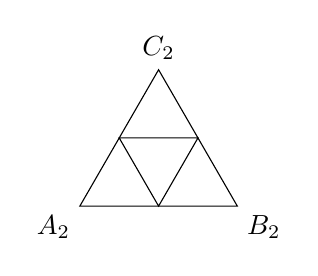
\begin{tikzpicture}[scale=2]
  \coordinate (A) at (0,0);
  \coordinate (B) at (1,0);
  \coordinate (C) at (0.5,{sqrt(3)/2});
  \recursiveTriangleQTwo{A}{B}{C}{1};
  \node[below left] at (A) {$A_2$};
  \node[below right] at (B) {$B_2$};
  \node[above] at (C) {$C_2$};
\end{tikzpicture}
\caption{図形 \( Q_2 \)}
\end{subfigure}
\hfill
% Q3
\begin{subfigure}[b]{0.22\textwidth}
\centering
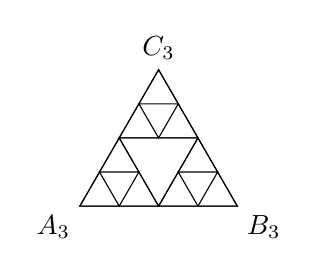
\begin{tikzpicture}[scale=2]
  \coordinate (A) at (0,0);
  \coordinate (B) at (1,0);
  \coordinate (C) at (0.5,{sqrt(3)/2});
  \recursiveTriangleQThree{A}{B}{C};
  \node[below left] at (A) {$A_3$};
  \node[below right] at (B) {$B_3$};
  \node[above] at (C) {$C_3$};
\end{tikzpicture}
\caption{図形 \( Q_3 \)}
\end{subfigure}
\hfill
% Q4
\begin{subfigure}[b]{0.28\textwidth}
\centering
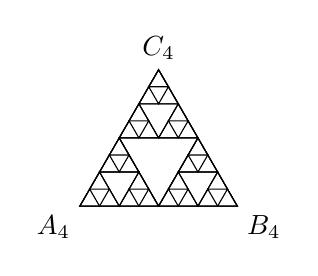
\begin{tikzpicture}[scale=2]
  \coordinate (A) at (0,0);
  \coordinate (B) at (1,0);
  \coordinate (C) at (0.5,{sqrt(3)/2});
  \recursiveTriangleQFour{A}{B}{C};
  \node[below left] at (A) {$A_4$};
  \node[below right] at (B) {$B_4$};
  \node[above] at (C) {$C_4$};
\end{tikzpicture}
\caption{図形 \( Q_4 \)}
\end{subfigure}

% \caption{再帰的に構成される三角形 \( Q_n \)}
\end{figure}


\end{document}